\noindent \textred{1.}
\textbf{(3 points)} \textit{Recurrences using RNNs}. Consider the recurrent network architecture below in \figref{fig:rnn}. All inputs are integers, hidden states are scalars, all biases are zero, and all weights are indicated by the numbers on the edges. The output unit performs binary classification. Assume that the input sequence is of \textbf{even} length. What is computed by the output unit at the final time step? Be precise in your answer. It may help to write out the recurrence clearly.

\begin{figure}[!h]
    \centering
    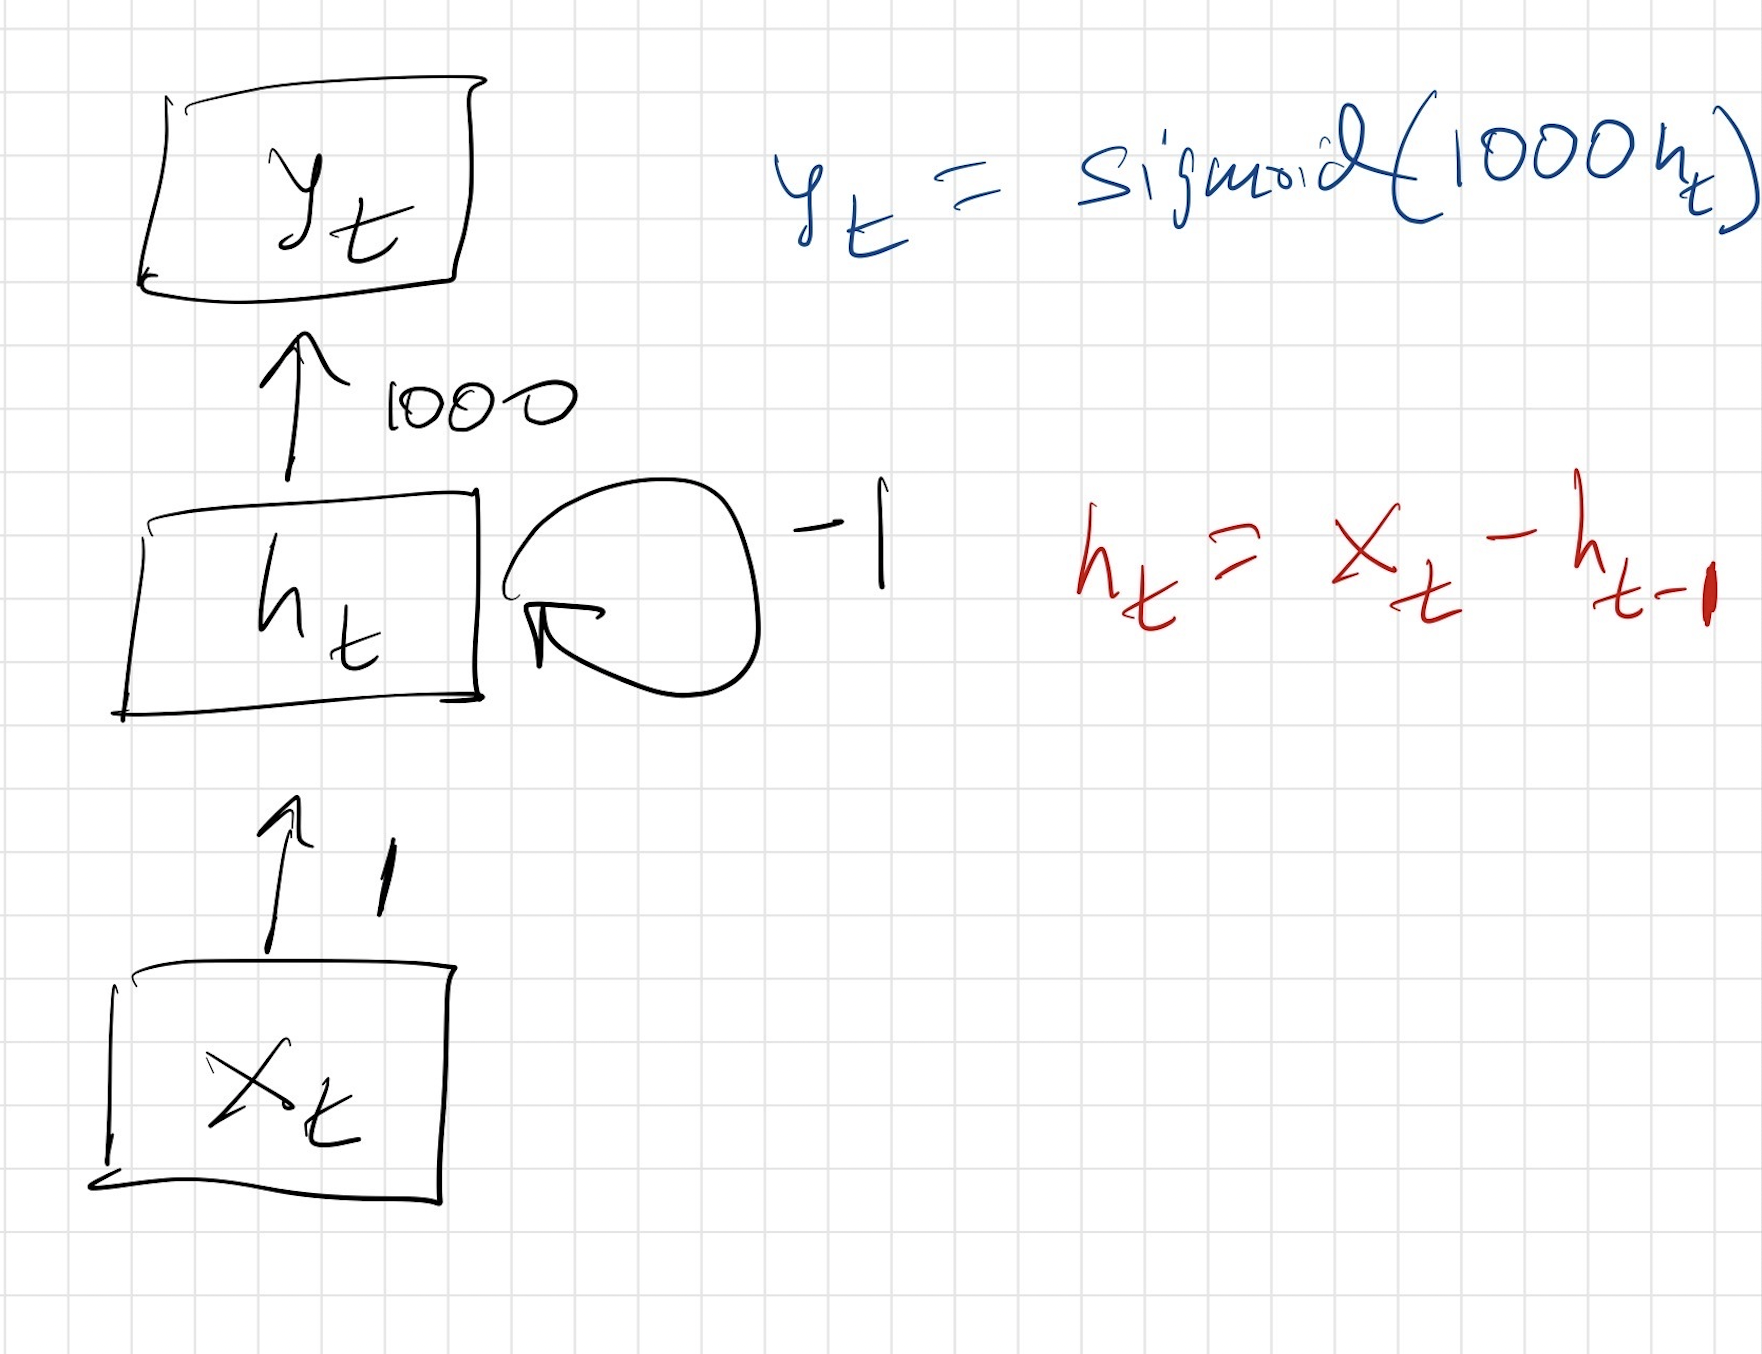
\includegraphics[width=0.5\linewidth]{HWs//HW2//figures/1.png}
    \caption{RNNs}
    \label{fig:rnn}
\end{figure}

\myAnswer{
Let inputs be $x_1, x_2, \dots, x_n$, where $n = 2k, k \in \mathbb{N}$, then all hidden states $h_i, i \in \mathbb{N}$ can be calculated as
\[
    h_i = \left\{
    \begin{array}{ccc}
        \sum_{j=1}^{i} (-1)^{j+1} x_j, & i = 2l+1 & (\text{odd}) \\
        \sum_{j=1}^{i} (-1)^{j} x_j, & i = 2l & (\text{even})
    \end{array}
    \right.
\]
Therefore, the output is
\[
    y_n = \mathrm{sigmoid}(1000 h_n) = \mathrm{sigmoid} \left( 1000 \sum_{j=1}^{n} (-1)^{j} x_j \right)
\]
}